\documentclass[a4paper, twocolumn]{article}
\usepackage[margin=0.8in]{geometry}
\usepackage{lmodern}
\usepackage{caption,setspace}
\usepackage{amssymb,amsmath}
\usepackage{ifxetex,ifluatex}
\usepackage[T1]{fontenc}
\usepackage[utf8]{inputenc}
\usepackage[unicode=true]{hyperref}
\usepackage{graphicx}
\usepackage{authblk}
\usepackage{eso-pic,lipsum}
% Massively reduces whitespace.
% \usepackage{savetrees}
% For tables.
\usepackage{booktabs}
\setlength{\heavyrulewidth}{1pt}
\setlength{\abovetopsep}{3pt}
% Increase space between columns.
\setlength\columnsep{20pt}
% For referencing.
\usepackage[backend=biber, natbib=true, style=numeric, sorting=none]{biblatex}
\addbibresource{write_up.bib}
% Make captions look different to regular text.
\captionsetup{font={footnotesize, sf}, labelfont=bf, width=\columnwidth}

\begin{document}
\title{\huge Latent Dimensionality Reduction: An Algorithmic Method for Interpreting Black Box Models \\
\Large \emph{DRAFT}}
\author{\emph{Elias Kassell, Fred Farrell}}
\date{September 2019}
\maketitle

\section{Abstract}\label{abstract}

LDR (Latent Dimensionality Reduction) is an algorithmic method for interpreting models by decomposing predictions from the original high dimensional feature space into a lower dimensional space. Both the output of the model and the certainty of its predictions are encoded in the condensed space. The method works out of the box on both classification and regression problems with input features relating to interpretable metrics. The output gives the ability to glimpse higher dimensional spaces, which are normally too complex for humans to understand, and is a powerful tool in understanding the underlying features generating the metrics.

\section*{Acknowledgements}

Thanks to Illumina\textsuperscript{\textregistered} for supporting this research. The extremely high dimensional problems posed by genomic analysis provided the inspiration for this work.

\section{Introduction}\label{Introduction}

When training a model to make predictions in situations where interpretability is not required, the main goal is to maximise predictive accuracy \cite{two-cultures}. Often black box models have a higher predictive accuracy than more interpretable solutions, particularly in higher dimensional or more complex problems \cite{deep-learning}. Because of the uninterpretability of these models, they become impractical for situations where it is a necessity to understand why a model has chosen a particular output as its prediction, and what effect changes to values of the input features will have on the output of the model.

Some examples of uses of model interpretation in real world applications include

\begin{enumerate}
\item Understanding the quality of a systems current understanding \cite{end-user-ml}. 

\item Interpreting how the value of a feature, or subset of features, affects a model's prediction (henceforth referred to as "feature interpretation"). For example, in a medical setting this interpretation can be used for suggesting the relation between features and a diagnosis. In another example, for manufacturing this interpretation can provide target values for the underlying processes involved in quality of produce.

\item The ability to use a model when not all values for the input features are present. By integrating across features which are not present, the certainty of a models prediction can be estimated. Current methods, such as imputing values for features which are not present, ignores the variability of the absent features across the feature space, which LDR can provide.
\end{enumerate}

\section{The Algorithm}

\begin{enumerate}
\item Normalize the original data so it falls into [0, 1] intervals.
\item Train a predictive model on the normalized data.
\item Train a OCSVM (One Class Support Vector Machine) \cite{ocsvm}, or an alternative model for detecting outliers, on the normalized data.
\item Create a KDE (kernel density estimate) \cite{kde} of the training points with a bandwidth equal to some resoltuion $r$. Optional: to improve the visualization, normalize the training to produce a constant density output.
\item Sample $n$ new points from the kernel density, using both classifiers to make predictions of each point. Weight the prediction according to the outlier classifier, where outliers have no model certainty in the prediction at that point.
\item Bin the samples according to regular intervals. For each dimension, group points with resolution $r$, reducing the value of the bin to the mean prediction across it.
\end{enumerate}

\section{Classification Example}

The Wisonsin breast cancer dataset \cite{breast-cancer} (provided by scikit \cite{scikit-learn}) is used as it has 31 dimensions, a significant number. The aim with the dataset is to classify the tumor as either malignant or benign. There are 569 samples in total, with 357 benign and 212 malignant.

\subsection{Random Forest and OCSVM Interpolation}

The 100 estimator RF (Random Forest) \cite{random-forest} achieved an F1 score of 0.975, while the OCSVM was trained to interpret 10\% of training values as outliers. Benign was selected as the positive category, resulting in a value of 1.0 indicating benign tumors and 0.0 inidicating malignant. All of the data is min-max scaled, then a 0.7/0.3 training/testing data split is applied. LDR is applied to the training data, integrating over 50,000 randomly selected points from the weighted kernel density of the sample space with a resolution of 1/50. Mean symmetry and mean area are selected for visual inspection of their individual effect on the model's classification. The certainty of the RF is shown in figure \ref{fig:interp-rf}, while the certianty of the OCSVM is shown in figure \ref{fig:interp-ocsvm}. The final combined certainty is shown in figure \ref{fig:interp-rf-ocsvm}.

\begin{figure}
\centering
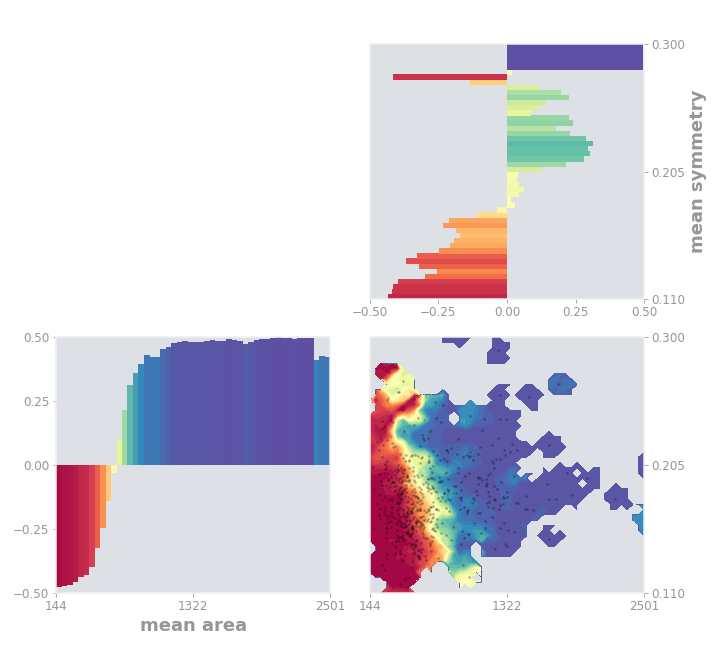
\includegraphics[width=0.8\columnwidth]{img/interp_rf.png}
\caption{RF prediction certainty, where red indicates certaincy of malignancy, blue certainty of benality, and yellow a general lack of certainty. A lack of drawn contour indicates no samples were drawn from the sample space, as the kernel density was too low in those areas. The black dots are the locations of the samples. The top and left axis are the single dimensional decomposition, while the bottom right is the two dimensional decomposition. In the single dimension estimates, the resulting value is shifted down by 0.5 to create a flat midpoint for the bars.}
\label{fig:interp-rf}
\end{figure}

\begin{figure}
\centering
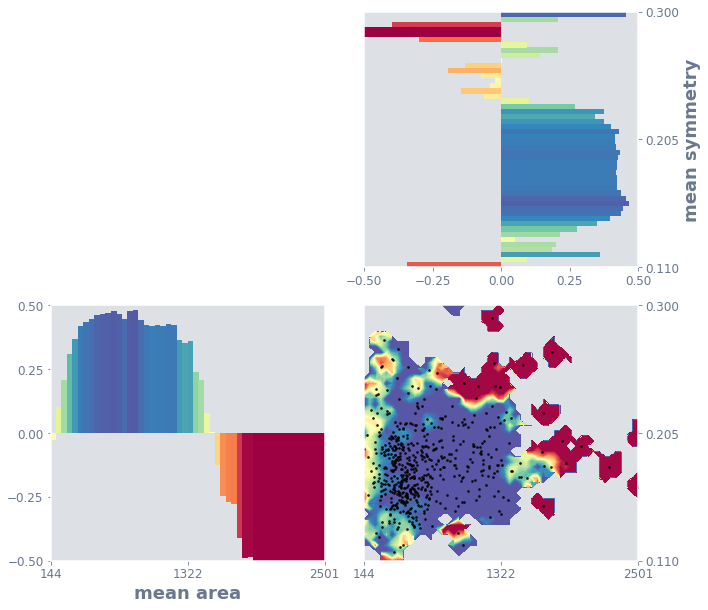
\includegraphics[width=0.8\columnwidth]{img/interp_ocsvm.png}
\caption{OCSVM prediction certainty, where red indicates certianty of outlier, blue certainty of not outlier, and yellow uncertainty.}
\label{fig:interp-ocsvm}
\end{figure}

\begin{figure}
\centering
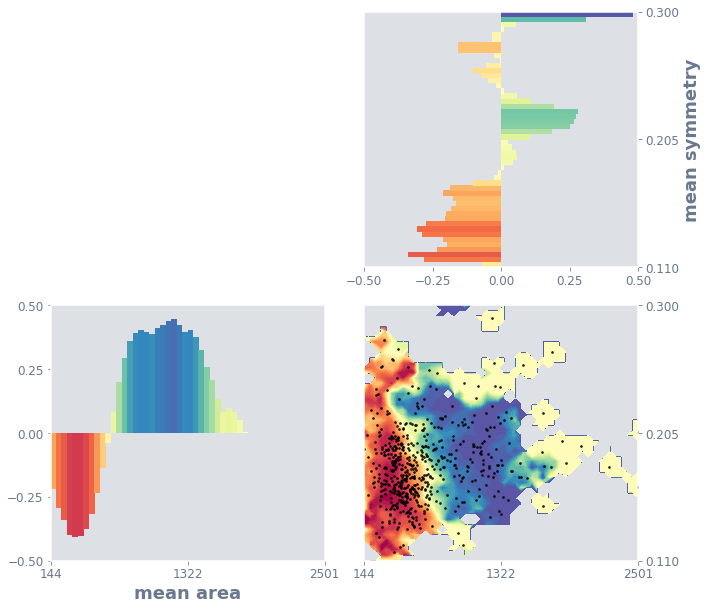
\includegraphics[width=0.8\columnwidth]{img/interp_rf_ocsvm.png}
\caption{RF with OCSVM interpolation prediction certainty, where red indicates overall certainty of malignancy, blue indicates overall certainty of benality, and yellow general overall uncertainty.}
\label{fig:interp-rf-ocsvm}
\end{figure}

\subsection{Neural Network and OCSVM Interpolation}

A 3 layer feed forward Neural Network (NN) was used (via pytorch \cite{paszke2017automatic}), consisting of an input layer, a hidden layer where tanh is applied, and an output layer. Softmax is applied when making predictions, and the final certainty of the prediction is calculated by calculating the proportion of the largest weighted class out of all weightings. The NN was trained over 50,000 epochs and achieved an F1 score of 0.961, slightly worse than the RF. The resulting LDR of the same features can be seen in figure \ref{fig:interp-nn-ocsvm}

\begin{figure}
\centering
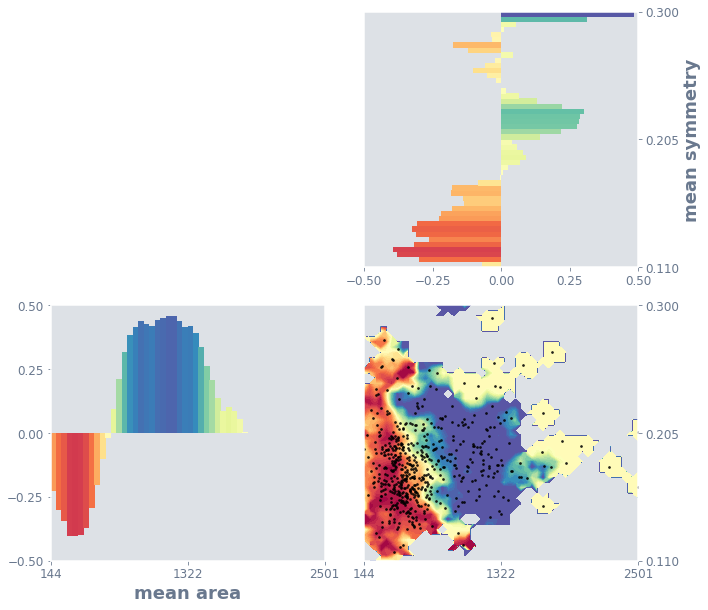
\includegraphics[width=0.8\columnwidth]{img/interp_nn_ocsvm.png}
\caption{NN with OCSVM interpolation prediction certanty.}
\label{fig:interp-nn-ocsvm}
\end{figure}

\subsection{Analysis of Discrepancy Between RF and NN}

There is very little discrepancy between the two LDR representations, both of which have similar predictive success. This is significant because random forests are widely regarded as more interpretable than neural networks \cite{random-forest-int}, but LDR represents them both in an equally interpretable fashion. The only visual difference between the two LDR representation arises from the NN tending to be more certain of its classifications. This can be seen in the scatter plots of prediction certainties for mean symmetry of the RF in figure \ref{fig:rf-ocsvm-mean-symmetry-scatter}m compared to the NN in figure \ref{fig:nn-ocsvm-mean-symmetry-scatter}.

\begin{figure}
\centering
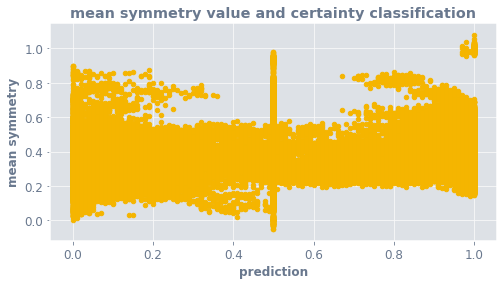
\includegraphics[width=0.7\columnwidth]{img/rf_ocsvm_mean_symmetry.png}
\caption{RF prediction certainty scatter plot of mean symmetry.}
\label{fig:rf-ocsvm-mean-symmetry-scatter}
\end{figure}

\begin{figure}
\centering
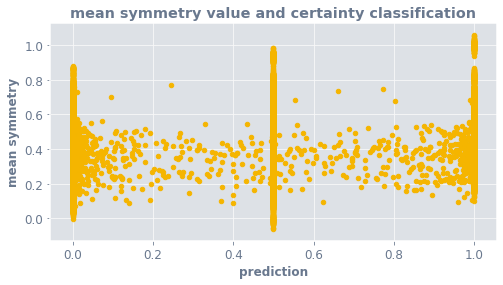
\includegraphics[width=0.7\columnwidth]{img/nn_ocsvm_mean_symmetry.png}
\caption{NN prediction certainty scatter plot of mean symmetry.}
\label{fig:nn-ocsvm-mean-symmetry-scatter}
\end{figure}

\section{Regression Example}

A similar method as with the classification was applied to the Boston House Price dataset \cite{boston-house} (also provided by scikit \cite{scikit-learn}). This dataset has 14 dimensions, where the target is to predict the house price based off of quantitative factors such as age of the house, the number of rooms, and the per capita crime rate of the time within which is situated. Some interesting relations are made immediately available from the LDR, shown in figure \ref{fig:reg-rf-ocsvm-matrix}, are

\begin{figure}
\centering
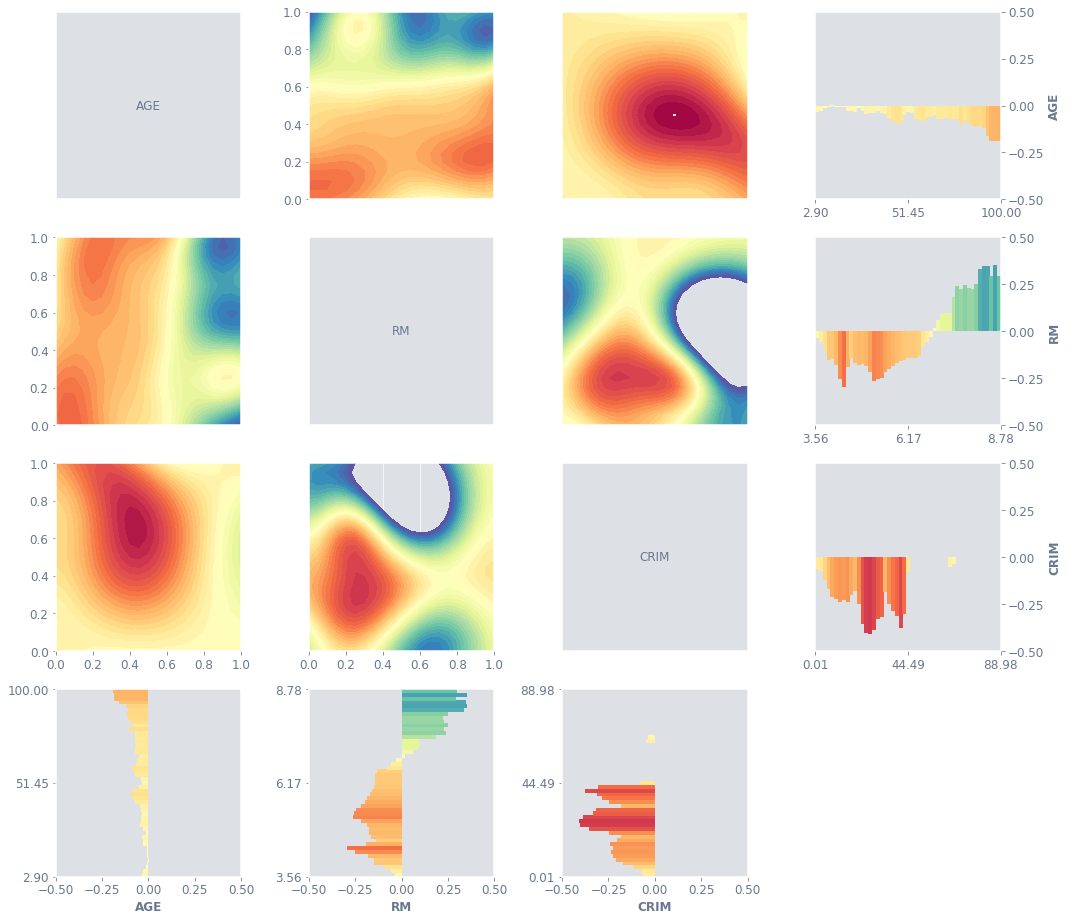
\includegraphics[width=\columnwidth]{img/reg_rf_ocsvm_matrix.png}
\caption{Regression RF with OCSVM interpolation. AGE is the age of the house, RM the number of rooms, and CRIM the per capita crime rate per town.}
\label{fig:reg-rf-ocsvm-matrix}
\end{figure}

\begin{enumerate}
\item An increasing crime rate tends to correlated with houses being worth less. Above the median level of crime however, the model becomes uncertain.
\item Any quantity of crime only has a negative effect on house price.
\item The lower the crime rate, the more rooms a house tends to have, and the more it is worth.
\item The older the house, the less it tends to be worth.
\item The age of the house and the number of rooms are for the most part independent.
\end{enumerate}

The prediction certainty prior to be binning can be seen in figure \ref{fig:reg-rf-ocsvm-rm}.

\begin{figure}
\centering
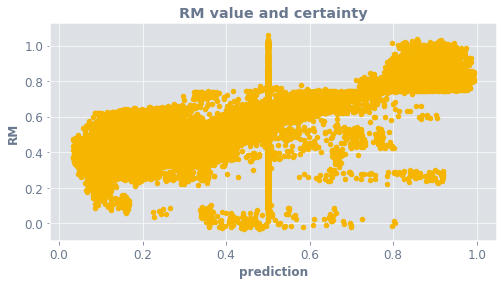
\includegraphics[width=0.7\columnwidth]{img/reg_rf_ocsvm_rm.png}
\caption{RF prediction certainty of number of rooms.}
\label{fig:reg-rf-ocsvm-rm}
\end{figure}

\section{Mathematical Explanation}

Let $\Omega$ be the total sample space of input data. Let $X \in \Omega$ describe an input vector of data of length $n$, where each $x_i \in [0, 1]$ is the scaled value for feature $i$ in the vector.

$$X = \{x_1, x_2, \ldots, x_n\}$$

Let $Y$ be a single or multivariate output vector ($Y = y$ if single) where each $y_i$ is a predicted variable.

$$Y = \{y_1, y_2, \ldots, y_n\}$$

Let $s \in [0, 1]$ be a prediction of an outlier, s.t. 1 indicates an outlier and 0 not an outlier.

Let $m$ describe a model as a function s.t. $m(X) = Y$, and $o$ describe an outlier classifier function s.t. $o(X) = s$

$$m(X) = Y$$

$$o(X) = s$$

Let the outlier weighting and model prediction interpolation function $f$ be defined as

$$f(X) = (m(X) - 0.5) \times o(X) + 0.5$$

Let the resolution of a KDE bandwidth be $r$. The KDE function $g$ over a $n$ samples can therefore be defined as

$$g(X) = \frac{1}{nr} \sum^n_{i=1} K \frac{(x - x_i)}{h}$$

which is effectively an implementation of the VEGAS algorithm for the Monte Carlo Integration function $I_\Omega$.

Let the set of points drawn from $\Omega$ be $Q$, where $q \in {i*r}^{1/r}_0$ while $x_i$ are drawn from $g$. $Q$ can therefore be described as

$$Q = {x_1, x_2, \ldots, q, \ldots, x_n}$$

One option for model certainty and outlier interpolation estimation is therefore given by

$$I_\Omega = \{\frac{1}{n} \sum^n_{i=1} f(Q(X))\}$$

While an alternative method is to use an SVM, or alternative predictive model, to model the function describing the dimensionality reduced space model certainty. Let this model be defined as $h$, resulting in

$$I_\Omega = h(Q(X))$$

\section{Conclusion}\label{Conclusion}

I have demonstrated that it is possible to interpret lower dimension subsets of high dimensional feature spaces by estimating the prediction of black box models trained on the feature spaces. However, before acceptance for clinical purposes, the model should be rigorously tested on more data sets. In addition to this, further research of extending LDR could be to interpret latent features that do not relate to uninterpretable input features, such as neural networks trained on images; a visualization of the prediction of the model based on a single pixel would not be of much use by itself.

\printbibliography

\end{document}